\begin{figure}
    \centering
    
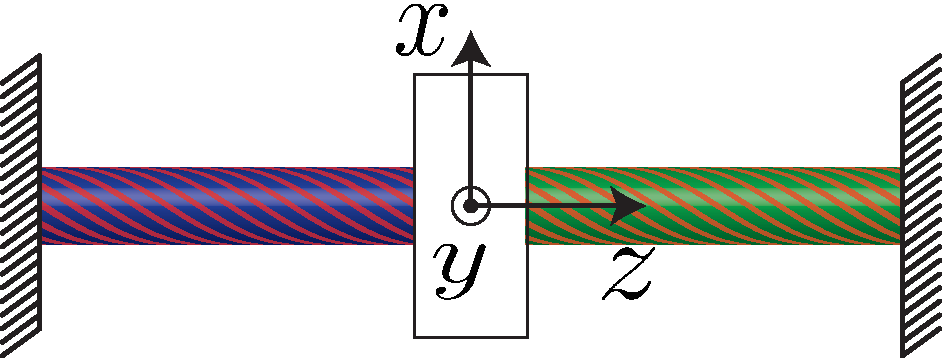
\includegraphics[width=0.6\linewidth]{figures/axesAligned_2par.pdf}
    
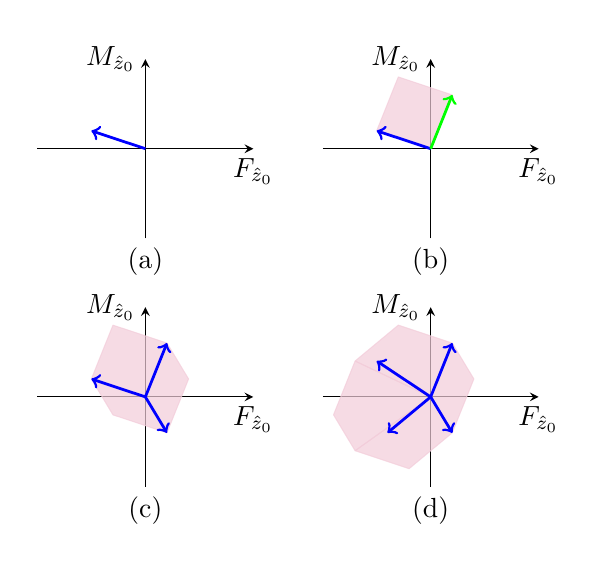
\begin{tikzpicture}
\matrix [row sep=0cm, column sep=0.5cm, style={align=center}] (my matrix) at (0,0)
{
% PLOT (a)
\begin{axis}[
    axis lines=center,
    xlabel={$F_{\hat{z}_0}$},
    ylabel={$M_{\hat{z}_0}$},
    ymin=-10, ymax=10, ytick={0}, ylabel near ticks,
    xmin=-10, xmax=10, xtick={0}, xticklabel=$\pgfmathprintnumber{\tick}^\circ$, xlabel near ticks, 
    xlabel style={at=(current axis.right of origin), anchor=north}, ylabel style={at=(current axis.above origin), anchor=east, rotate=-90},
    scale=0.4,
    anchor=center,
]
    \addplot [->, line width=1pt, blue] coordinates {(0,0) (-5,2)};
\end{axis};
&
% PLOT (b)
\begin{axis}[
    axis lines=center,
    xlabel={$F_{\hat{z}_0}$},
    ylabel={$M_{\hat{z}_0}$},
    ymin=-10, ymax=10, ytick={0}, ylabel near ticks,
    xmin=-10, xmax=10, xtick={0}, xticklabel=$\pgfmathprintnumber{\tick}^\circ$, xlabel near ticks, 
    xlabel style={at=(current axis.right of origin), anchor=north}, ylabel style={at=(current axis.above origin), anchor=east, rotate=-90},
    scale=0.4,
    anchor=center,
]
    \addplot[patch, opacity=0.7, fill=purple!20, faceted color=purple!20, patch type=rectangle] 
        coordinates {(0,0) (-5,2) (-3,8) (2,6)};
    \addplot [->, line width=1pt, blue] coordinates {(0,0) (-5,2)};
    \addplot [->, line width=1pt, green] coordinates {(0,0) (2,6)};
\end{axis};
\\
\node (a) {(a)}; & \node (b) {(b)};
\\
% PLOT (c)
\begin{axis}[
    axis lines=center,
    xlabel={$F_{\hat{z}_0}$},
    ylabel={$M_{\hat{z}_0}$},
    ymin=-10, ymax=10, ytick={0}, ylabel near ticks,
    xmin=-10, xmax=10, xtick={0}, xticklabel=$\pgfmathprintnumber{\tick}^\circ$, xlabel near ticks, 
    xlabel style={at=(current axis.right of origin), anchor=north}, ylabel style={at=(current axis.above origin), anchor=east, rotate=-90},
    scale=0.4,
    anchor=center,
]
    \addplot[patch, opacity=0.7, fill=purple!20, faceted color=purple!20, patch type=rectangle] 
        coordinates{
                    (0,0) (-5,2) (-3,8) (2,6)
                    (0,0) (2,6) (4,2) (2,-4)
                    (0,0) (2,-4) (-3,-2) (-5,2)
                    };
    \addplot [->, line width=1pt, blue] coordinates {(0,0) (-5,2)};
    \addplot [->, line width=1pt, blue] coordinates {(0,0) (2,6)};
    \addplot [->, line width=1pt, blue] coordinates {(0,0) (2,-4)};
\end{axis};
&
% PLOT (d)
\begin{axis}[
    axis lines=center,
    xlabel={$F_{\hat{z}_0}$},
    ylabel={$M_{\hat{z}_0}$},
    ymin=-10, ymax=10, ytick={0}, ylabel near ticks,
    xmin=-10, xmax=10, xtick={0}, xticklabel=$\pgfmathprintnumber{\tick}^\circ$, xlabel near ticks, 
    xlabel style={at=(current axis.right of origin), anchor=north}, ylabel style={at=(current axis.above origin), anchor=east, rotate=-90},
    scale=0.4,
    anchor=center,
]
    \addplot[patch, opacity=0.7, fill=purple!20, faceted color=purple!20, patch type=rectangle] 
        coordinates {
                    (0,0) (-7,4) (-3,8) (2,6)
                    (0,0) (2,6) (4,2) (2,-4)
                    (0,0) (2,-4) (-2,-8) (-7,-6)
                    (0,0) (-7,-6) (-9,-2) (-7,4)
                    };
    \addplot [->, line width=1pt, blue] coordinates {(0,0) (-5,4)};
    \addplot [->, line width=1pt, blue] coordinates {(0,0) (-4,-4)};
    \addplot [->, line width=1pt, blue] coordinates {(0,0) (2,6)};
    \addplot [->, line width=1pt, blue] coordinates {(0,0) (2,-4)};
\end{axis};
\\
%% PLOT (d)
%\begin{axis}[
%    axis lines=center,
%    xlabel={$F$},
%    ylabel={$M$},
%    ymin=-10, ymax=10, ytick={0}, ylabel near ticks,
%    xmin=-10, xmax=10, xtick={0}, xticklabel=$\pgfmathprintnumber{\tick}^\circ$, xlabel near ticks, 
%    xlabel style={at=(current axis.right of origin), anchor=north}, ylabel style={at=(current axis.above origin), anchor=east, rotate=-90},
%    scale=0.4,
%    anchor=center,
%]
%    \addplot[patch, opacity=0.7, fill=purple!20, faceted color=purple!20, patch type=rectangle] 
%        coordinates{
%                    (0,0) (-4,4) (-8,0) (-4,-4)
%                    (0,0) (-4,4) (0,4) (4,0)
%                    (0,0) (-4,-4) (0,-4) (4,0)
%                    };
%    \addplot [->, line width=1pt, blue] coordinates {(0,0) (-4,4)};
%    \addplot [->, line width=1pt, blue] coordinates {(0,0) (-4,-4)};
%    \addplot [->, line width=1pt, blue] coordinates {(0,0) (4,0)};
%\end{axis};
%\\
\node (c) {(c)}; & \node (d) {(d)};
\\
};
\end{tikzpicture}

    \caption{Examples of force polygons for axis-aligned parallel combinations of (a) 1 FREE, (b) 2 FREEs, (c) 3 FREEs, (d) 4 FREEs.}
    \label{fig:cvxHull}
\end{figure}